\chapter{Východiská}
\label{kap:vyc} % id kapitoly pre prikaz ref

\section{Úvod do problematiky}

Problém hľadania optimálnej cesty je veľmi rozšíreným problémom nie len v doprave. Doteraz bolo navrhnutých množstvo algoritmov, metód a techník na vyriešenie tohto problému. Pri hľadaní optimálnej trasy vo verejnej doprave je dobré si najskôr ujasniť, čo  výraz optimálna csesta znamená.

Najlepšie zhrnutie podproblémov, ktoré môžu nastať sme postrehli v článku \cite{circular}. 
Autori analyzujú ich návrh v najzložitejšom systéme verejnej dopravy - v Hongkongu. Pre verejnú dopravu je praktickejšie navrhnúť viac alternatívnych ciest. Najbežnejšie používateľské preferencie sú:
\begin{itemize}
\item{minimálny čas}
\item{minimálne poplatky}
\item{minimálny počet prestupov}
\item{minimálna vzdialenosť peších prestupov}
\end{itemize}
Ďalej si treba uvedomiť, že môžu existovať rôzne typy liniek - jednosmerné alebo okružné a taktiež linky závislé na čase - denné, nočné alebo víkendové linky. Vzhľadom na rôzne požiadavky existuje viacero potenciálnych riešení. Neexistuje totiž všeobecne dokonalý spôsob na hľadanie optimálnej cesty, ktorý sedí pre každú verejnú dopravu, najmä kvôli rozloženiu zastávok.

Bratislavská verejná doprava má rôzne typy dopravných prostriedkov (autobus, trolejbus a električka), čo tiež predstavuje určitý problém. Pri prestupoch treba zohľadniť aj pešie presuny. Dopravná sieť, ktorú budeme modelovať v našej práci je teda multimodálna. Multimodálna sieť je definovaná ako kombinácia dvoch a viacerých dopravných prostriedkov na prepravu cestujúcich alebo tovaru z počiatočného miesta na miesto určenia \cite{timedependent}.

Ďalším kľúčovým problémom sú podľa zadania reálne dáta. Bude potrebné vyriešiť, ako sa vysporiadať so spracovaním reálnych dát. Kľúčový bude výber dátovej štruktúry na ich spracovanie, ako aj nájdenie vhodného časovo závislého algoritmu.

Sumarizáciou nášho problému je, ako sa vysporiadať s dynamickými dátami, alternatívnymi cestami, viacerými módmi, navigáciou z iného miesta ako zo zastávky. Ďalej chceme vyhovieť používateľským preferenciám, ako je minimálny čas, minimálny počet prestupov a minimálna vzdialenosť peších prestupov. Neposledným problémom je návrh architektúry systému.

V tejto kapitole ďalej opíšeme často skloňované algoritmy pri téme multimodálneho časovo závislého vyhľadávania vo verejnej doprave a priblížime výskumy, ktoré riešili podobné problémy ako my.

\section{Známe algoritmy hľadania najkratšej cesty}
\subsection{Dijkstrov algoritmus}
Najznámejším algoritmom hľadania najkratšej cesty v orientovanom, kladne ohodnotenom grafe je Dijkstrov algoritmus. Algoritmus vie nájsť najrýchlejšiu cestu medzi dvomi danými vrcholmi. Známejšou verziou Dijkstrovho algoritmu je hľadanie najkratšej cesty z jedného vrcholu do všetkých ostatných vrcholov v grafe. 

Rozhodujúcou hodnotou je vzdialenosť vrcholu $d(n)$, ktorá predstavuje dĺžku cesty od začiatočného vrcholu po vrchol $n$, pričom cesta vedie cez aktuálny vrchol.
Pre začiatočný vrchol sa vzdialenosť $d(n) = 0$ a všetky ostatné vrcholy majú hodnotu $d(n) = \infty$. Na začiatku je začiatočný vrchol označený ako aktuálny. Pri každej iterácii algoritmus preskúma všetky susedné vrcholy aktuálneho vrcholu. Pre každý susedný vrchol prepočíta hodnotu $d(n)$. Ak je táto hodnota menšia ako predtým zaznamenaná, prepíše ju menšou hodnotou. Ďalej algoritmus označí aktuálny vrchol ako navštívený. Tým pádom sa tento vrchol už nebude viac prehľadávať. Aktuálnym vrcholom sa stane zatiaľ nenavštívený vrchol s najmenšou hodnotou $d(n)$. 

Ak hľadáme cestu medzi dvomi konkrétnymi vrcholmi, algoritmus končí, keď bol konečný vrchol označený ako navštívený. Inak končí, ak neexistujú žiadne nenavštívené vrcholy alebo majú všetky hodnotu $d(n) = \infty$.

Časová zložitosť Dijkstrovho algoritmu je kvadratická
$\mathcal{O}(|V|)$, kde $V$ je množina všetkých vrcholov v grafe. V pôvodnej verzii, kde hľadáme najkratšiu cestu len medzi dvomi vrcholmi, môže algoritmus bežať rýchlejšie.

Nevýhodou algoritmu je veľký prehľadávaný priestor. Existuje viacero algoritmov, ktoré vznikli modifikáciou Dijkstrovho algoritmu. Napríklad Bellman-Fordov algoritmus, ktorý sa vie vysporiadať aj so zápornými hranami alebo A*, ktorý využíva heuristiku na zmenšenie prehľadávaného priestoru. 

\subsection{A* algoritmus}
A* algoritmus je grafový optimálny algoritmus na nájdenie najkratšej cesty medzi dvoma bodmi. Vznikol kombináciou heuristických a formálnych prístupov. Udržuje strom ciest začínajúcich v koreni stromu a predlžuje tieto cesty po jednej hrane. Pri každej iterácii sa rozhodne, ktorú z ciest rozšíri. Algoritmus sa skončí, ak už neexistuje žiadna cesta na rozšírenie alebo pri dosiahnutí koncového vrcholu. Pri prehľadávaní používa stratégiu najskôr najlepšieho. Heuristika, ktorá sa využíva na vyhodnotenie vzdialeností, je funkcia
\begin{equation}
f(n) = g(n) + h(n), 
\end{equation}
kde $g(n)$ predstavuje hodnotu cesty zo začiatočného vrcholu do vrcholu $n$ a $h(n)$ je heuristická funkcia, ktorá odhaduje najkratšiu cestu z vrcholu $n$ do koncového vrcholu.

Najčastejšie používaná heuristická funkcia na odhadovanie vzdialenosti je Euklidovská vzdialenosť.
Heuristika je prípustná, ak nikdy neprecení skutočné náklady na dosiahnutie cieľa. Potom je zaručené, že algoritmus A* vráti najkratšiu cestu, ak taká v grafe existuje.

Časová zložitosť A* algoritmu závisí od zvolenej heuristiky. V najhoršom prípade je zložitosť algoritmu exponenciálna, v najlepšom prípade môže byť polynomiálna.

\section{Časovo závislý algoritmus}
Stretávame sa s problémom, kedy ohodnotenie hrán v grafe nie je konštantné, ale je závislé od času. Boli navrhnuté rôzne riešenia, ako ohodnotiť hrany, aby sa na model dal aplikovať niektorý z klasických algoritmov hľadania najkratšej cesty. 

V článku \cite{trains} tvrdia, že ak dokážeme odhadnúť hodnotu hrany konštantným číslom, potom riešenie klasického problému hľadania najkratšej cesty môže fungovať ako heuristické riešenie problému najkratšej cesty závislej od stavu.

Ďalšia navrhovaná metóda je založena na stochastickom čase jazdy. V článku \cite{stochastic} používajú Bayesovu formulu na získanie prevdepodobnostného rozdelenia času cestého úseku. Na hľadanie optimálnej trasy navrhli a následne použili genetické algoritmy.

\subsection{Multimodálny algoritmus}
Článok \cite{timedependent} navrhuje časovo závislý algoritmus hľadania najkratšej cesty pre multimodálnu dopravnú sieť, pričom využíva A* algoritmus. Navrhnutý algoritmus hľadá len jednu cestu medzi začiatočným a koncovým vrcholom. 

Autori definujú graf $G = (V, E, M, T)$ ako multimodálny časovo závislý graf, kde $V$ je množina vrcholov, $E$ je množina hrán, $M$ je množina módov a $T$ je množina jázd.
Hrana $e_i = (v_i, v_j, m_i)$ je cesta z vrcholu $v_i$ do $v_j$ použitím módu $m_i$. Vrchol, kde sa menia módy je prestupný vrchol. Ďalej definujú čas prestupu ako súčet:
\begin{itemize}
\item{času potrebného na prestup medzi dvomi zastávkami}
\item{času potrebného na čakanie na prestupný mód}
\item{času, ktorý stojí mód na zastávke (týka sa skôr prímestskej dopravy)}
\end{itemize}

Preto je potrebné pridať ďalšie prestupné hrany s tým, že ohodnotenie hrán nebude statické, ale bude to funkcia $cost_{transfer}()$ závislá od času.

Nech hrana $e = (v, v’)_m$ má časovo závislú hodnotu $c_e(t)$, jazda pre hranu $e$ je definovaná ako dvojica $travel_e = (t, t’)$, kde $t$ je čas odchodu z $v$ a $t’$ je čas príchodu do $v’$.

\section{Spracovanie reálnych dát}
\label{sec:models}
Verejná doprava má časté meškania spojov z dôvodu nehôd, rôznych porúch spojov alebo servisných prác. Takéto situácie spôsobujú problémy vo verejnej doprave, ale aj pri navrhovaní systému. Aby boli používateľom poskytnuté čo najoptimálnejšie trasy, potrebujeme reálne dáta o polohe vozidiel.

Tieto dáta môžeme získať v rôznej forme. Ak by našimi dátami bola pozícii vozidla z GPS, potrebujeme získané pozície vozidiel nejakým spôsobom spracovať. V článku \cite{mapmatching} navrhujú, ako spracovať takto získané dáta. Proces \textit{map-matching} je navrhnutá metóda integrácie údajov z digitálnych máp s údajmi z polohovacieho systému (GPS). Tento proces slúži na identifikáciu správnej linky, po ktorej vozidlo ide a na určenie presnej polohy tohto vozidla v rámci linky.

Ak už dáta máme spracované, potrebujeme model, na ktorom bude časovo-závislý algoritmus bežať. Na vytvorenie modelu boli v článku \cite{models} navrhnuté 2 prístupy: time-expanded model a time-dependent model.

\subsection{Time-expanded model}
\textit{Time-expanded} model rozdelí čas na konečný počet intervalov a pre každý interval zduplikuje vrchol. Každá udalosť na každej stanici je modelovaná ako vrchol. Model je vhodný pre siete založené na cestovných poriadkoch. Je teda vhodný pre verejnú dopravu. Ľahko sa modeluje, ale vyžaduje veľa pamäte a vykonávanie dotazov je pomalé.

\subsection{Time-dependent model}
\textit{Time-dependent} model má klasickú topológiu. Počet vrcholov vo výslednom modeli je rádovo menší ako v \textit{time-expanded} modeli. Okrem iného je tento model aj efektívnejší. 

Pre každú zastávku $p$ je do modelu vložený \textit{station node}. Navyše pre každú zastávku $p$ v linke $r$ je vytvorený ďalší vrchol \textit{route node} $r_p$. \textit{Route nodes} sú spojené so \textit{stations nodes} hranami s konštantným ohodnotením. Toto ohodnotenie predstavuje čas potrebný na prestup. Jazda vozidla \textit{t} je definovaná ako postupnosť zastávok, ktoré vozidlo navštevuje podľa daného cestovného poriadku. Jazdy, ktoré pozostávajú z rovnakých vrcholov sú zoskupené do liniek. \textit{Route nodes}, ktoré patria jednej linke sú spojené hranou , ktorej hodnotou je funkcia. Hoci je takto vytvorený model menší, pre algoritmy je komplikovanejší. Ťažko sa na ňom vykonávajú dotazy v prípade, že je potrebné brať do úvahy prestupy.


\section{Optimalizačné metódy}
\label{sec:optimalization}
V tejto sekcii spomenieme optimalizačné metódy, ktoré minimalizujú prehľadávanie, aby algoritmy hľadania najkratšej cesty bežali rýchlejšie a efektívnejšie. Jedna z metód, ktorá sa dá použiť na grafe, ktorého vrcholy nemajú reálne súradnice, je algoritmus spomínaný v článku \textit{IBAS - Index-Based A-Star}. Autori navrhli heuristiku, ktorá používa 3 indexy na určenie a odrezanie nepotrebných vrcholov pre výpočet najkratšej cesty. Ak poznáme reálne súradnice vrcholov, je efektívnejšie využiť niektoré z techník minimalizácie prehľadávaného priestoru.

\subsection{Minimalizácia prehľadávaného priestoru v okolí virtuálnej cesty}

V článku \cite{timedependent} navrhujú optimalizáciu A* algoritmu založenú na vypočítaní virtuálnej cesty, ktorá predstavuje Euklidovskú vzdialenosť zo začiatočného do koncového vrcholu. Algoritmus hľadá cestu cez vrcholy, ktoré sú blízko virtuálnej cesty. 

Definujeme parametre:
\begin{itemize}
\item{virtuálna cesta ($st$) – Euklidovská vzdialenosť z $s$ do $t$} a zároveň dolné ohraničenie prehľadávaného priestoru
\item{vzdialenosť $d$ - priemerná vzdialenosť všetkých vrcholov k virtuálnej ceste a predstavuje horné ohraničenie prehľadávaného priestoru}
\item{$d_{max}$ – vzdialenosť najvzdialenejšieho vrcholu od virtuálnej cesty}
\item{$\Delta d$ – priemerná vzdialenosť od všetkých vrcholov ku všetkým susedom}
\end{itemize}

Algoritmus funguje nasledovne:
\begin{enumerate}
\item Vypočítame: $D = dist(s,t)$, $d$ a $\Delta d$. Prehľadávaný priestor ma rozmery $(2d,D)$.
\item Začneme vytvárať cestu tak, že hľadáme vrchol $v_i$, ktorý spĺňa podmienku \\$dist(v_i, st) \leq d$. Ak nevieme nájsť žiadneho takého kandidáta, navyšujeme $d$ o $\Delta d$, až kým nejakého nenájdeme.
\item V každej ďalšej iterácii po výbere vrcholu $v_i$ hľadáme ďalšieho kandidáta.
\item Ak sme prehľadali všetky vrcholy v grafe a nezostavili sme najkratšiu cestu, začneme prehľadávať odznovu s väčším prehľadávaným priestorom.
\end{enumerate}

\subsection{Minimalizácia prehľadávaného priestoru bounding boxom}
V článku \cite{alternate} sa autori snažia nájsť spôsob, ako efektívne vypočítať najkratšiu cestu a tak odľahčiť cesty od dopravných zápch. Navrhujú algoritmus na nájdenie najkratšej alternatívnej cesty s minimálnym potrebným výpočtovým časom. 

Pre nás zaujímavý je ich prístup k vyhodnoteniu najkratšej cesty a k minimalizácii grafu. Minimalizácia grafu prebieha nepretržite. Vždy, keď zvažujeme ďalší susedný vrchol, definujeme nový \textit{bounding box} a tým odstránime nadbytočné vrcholy, ktoré pri výpočte nie sú relevantné.

Na začiatku potrebujeme vymodelovať graf mesta, kde sú vrcholy popísané zemepisnou šírkou a výškou a hrany sú ohodnotené reálnou vzdialenosťou medzi jednotlivými vrcholmi. Graf je opísaný tabuľkovou maticou a reprezentovaný graficky. Keď poznáme začiatočný a koncový vrchol, vytvoríme si tabuľku všetkých vrcholov, ich súradníc a vzdialeností do začiatočného vrcholu a koncového vrcholu. Podľa súradníc vieme vypočítať vzdialenosti medzi jednotlivými vrcholmi. Následne vygenerujeme grafickú reprezentáciu tejto tabuľky. 

\subsubsection{Bounding box}
Majme dopravnú sieť tvorenú 26 vrcholmi a majme začiatočný a koncový vrchol. \textit{Bounding box} je na začiatku vytvorený medzi začiatočným a koncovým vrcholom, ako je ukázané na obrázku \ref{fig:boundingBoxReal}. \textit{Bounding box} zredukuje sieť na 8 vrcholov, čím zredukuje prehľadávaný priestor, výpočtovú cenu a čas. Ďalšiu redukciu vieme dosiahnuť, ak nakloníme bounding box tým spôsobom, že spojnica začiatočného a koncového vrcholu bude osou boxu, ako môžeme vidieť na obrázku \ref{fig:boundingBoxRect}. 

\begin{figure}[H]
\centering
	\begin{subfigure}[b]{0.48\textwidth}
		\centering
 		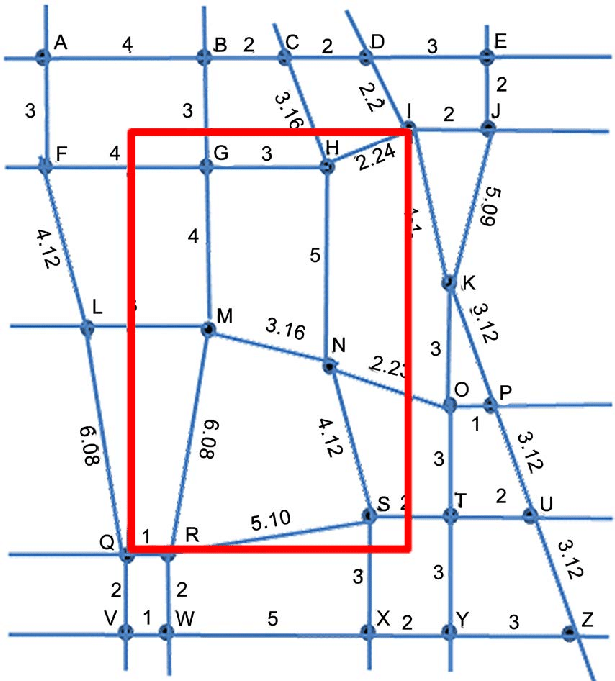
\includegraphics[width=0.9\linewidth]{images/bounding-box}
		\caption{Bounding box}
		\label{fig:boundingBoxReal}
	\end{subfigure}
	\begin{subfigure}[b]{0.48\textwidth}
		\centering
		\includegraphics[width=0.9\linewidth]{images/bounding-box-rect}
			\caption{Naklonený bounding box}
		\label{fig:boundingBoxRect}
	\end{subfigure}
	\caption[Bounding box]{}
	\label{fig:boundingBox}
\end{figure}

\begin{footnotesize}
Zdroj: Shortest Alternate Path Discovery through Recursive Bounding Box Pruning: Figure 5, Figure 13. Január 2017 [citované 18.8.2019]. Dostupné z \url{https://www.researchgate.net/publication/316188932_Shortest_Alternate_Path_Discovery_through_Recursive_Bounding_Box_Pruning}
\end{footnotesize}

\subsubsection{Navrhovaný algoritmus}
Dvojdimenzionálne súradnice v dopravnej sieti pomôžu určiť, či daný vrchol konverguje ku koncovému vrcholu alebo nie. 

Na začiatku vytvoríme \textit{bounding box} medzi začiatočným a koncovým vrcholom. Získame susedné vrcholy začiatočného vrcholu a pre všetky susedné vrcholy vypočítame vzdialenosť $d$. Vzdialenosť $d$ je rovná súčtu vzdialenosti medzi začiatočným vrcholom a daným susedným vrcholom a karteziánskou vzdialenosťou daného susedného vrcholu od koncového vrcholu. Zo susedných vrcholov je vybraný taký vrchol, ktorého hodnota $d$ je najmenšia. 

Nový vrchol sa stane začiatočným vrcholom a \textit{bounding box} sa znovu vygeneruje. Proces hľadania najbližšieho vrcholu pokračuje, kým sa najbližší vybraný vrchol nestane koncovým vrcholom. Týmto spôsobom nájdeme najkratšiu cestu. 

Následne vrcholy, ktoré sme nevyhodnotili, vyhodnotíme rovnakým spôsobom. Keď algoritmus spracuje všetky vrcholy, výsledok uloží vo vzostupnom poradí podľa veľkosti. Takto získame okrem najkratšej cesty aj alternatívne najkratšie cesty, viď obrázok \ref{fig:boundingBoxResult}. Na záver vymeníme začiatočný vrchol s koncovým vrcholom a výsledné polia spolu zjednotíme, aby sme získali čo najlepší výsledok. V prípade, že sa algoritmu nepodarí nájsť najkratšiu cestu, rozšírime \textit{bounding box}. Maximálna výpočtová cena tohto algoritmu je $7 \cdot \sqrt{2}N$.

\begin{figure}[H]
\centerline{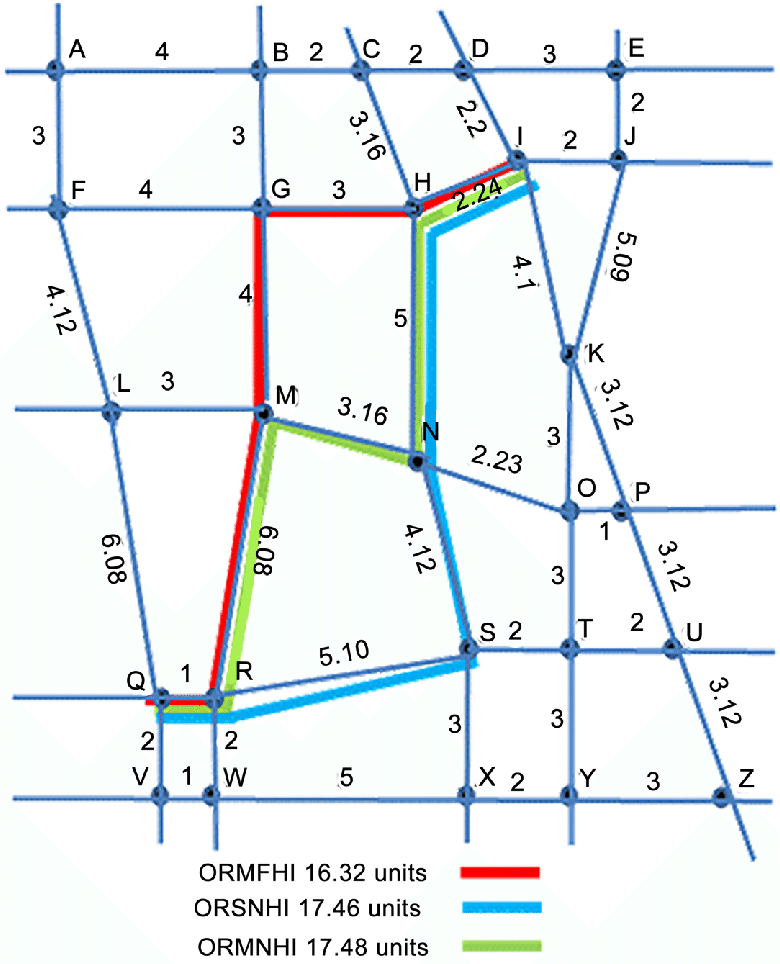
\includegraphics[width=0.4\textwidth]{images/bounding-box-result}}
\caption[Bounding box: 3 najkratšie cesty]{Bounding box: 3 najkratšie cesty}
\label{fig:boundingBoxResult}
\end{figure}

\begin{footnotesize}
Zdroj: Shortest Alternate Path Discovery through Recursive Bounding Box Pruning: Figure 5, Figure 12. Január 2017 [citované 18.8.2019]. Dostupné z \url{https://www.researchgate.net/publication/316188932_Shortest_Alternate_Path_Discovery_through_Recursive_Bounding_Box_Pruning}
\end{footnotesize}

\section{Zohľadnenie zadania polohy mimo zastávky}
\label{sec:actual-location}
V článku \cite{circular} autori poukazujú na to, že správny systém na hľadanie optimálnej trasy vo verejnej doprave by mal ponúknuť používateľovi možnosť vyhľadať trasu z miesta (prípadne na miesto), ktoré nie je nutne zastávkou. Ak hľadáme najkratšiu cestu z takto zadaného vrcholu, prvým krokom bude nájdenie prvej zastávky. Autori upozorňujú na to, že vyhľadanie najbližšej zastávky k danej pozícii nemusí byť správnym riešením.

Navrhovaným riešením je nájsť viacero zastávok radiálnym vyhľadávaním, ktorému určíme polomer. Vo vybranej zóne sa môže nachádzať viac zastávok, ktoré prislúchajú tej istej trase, ako môžeme vidieť na obrázku \ref{fig:circularRoute}. V tomto prípade by výber zastávky č. 2 (najbližšej zastávky k zadanej pozícii) nebol optimálny. Rovnako aj výberom zastávky č. 6 ako konečnej zastávky by nebolo súčasťou správneho riešenia hľadania najkratšej cesty. 

\begin{figure}[H]
\centerline{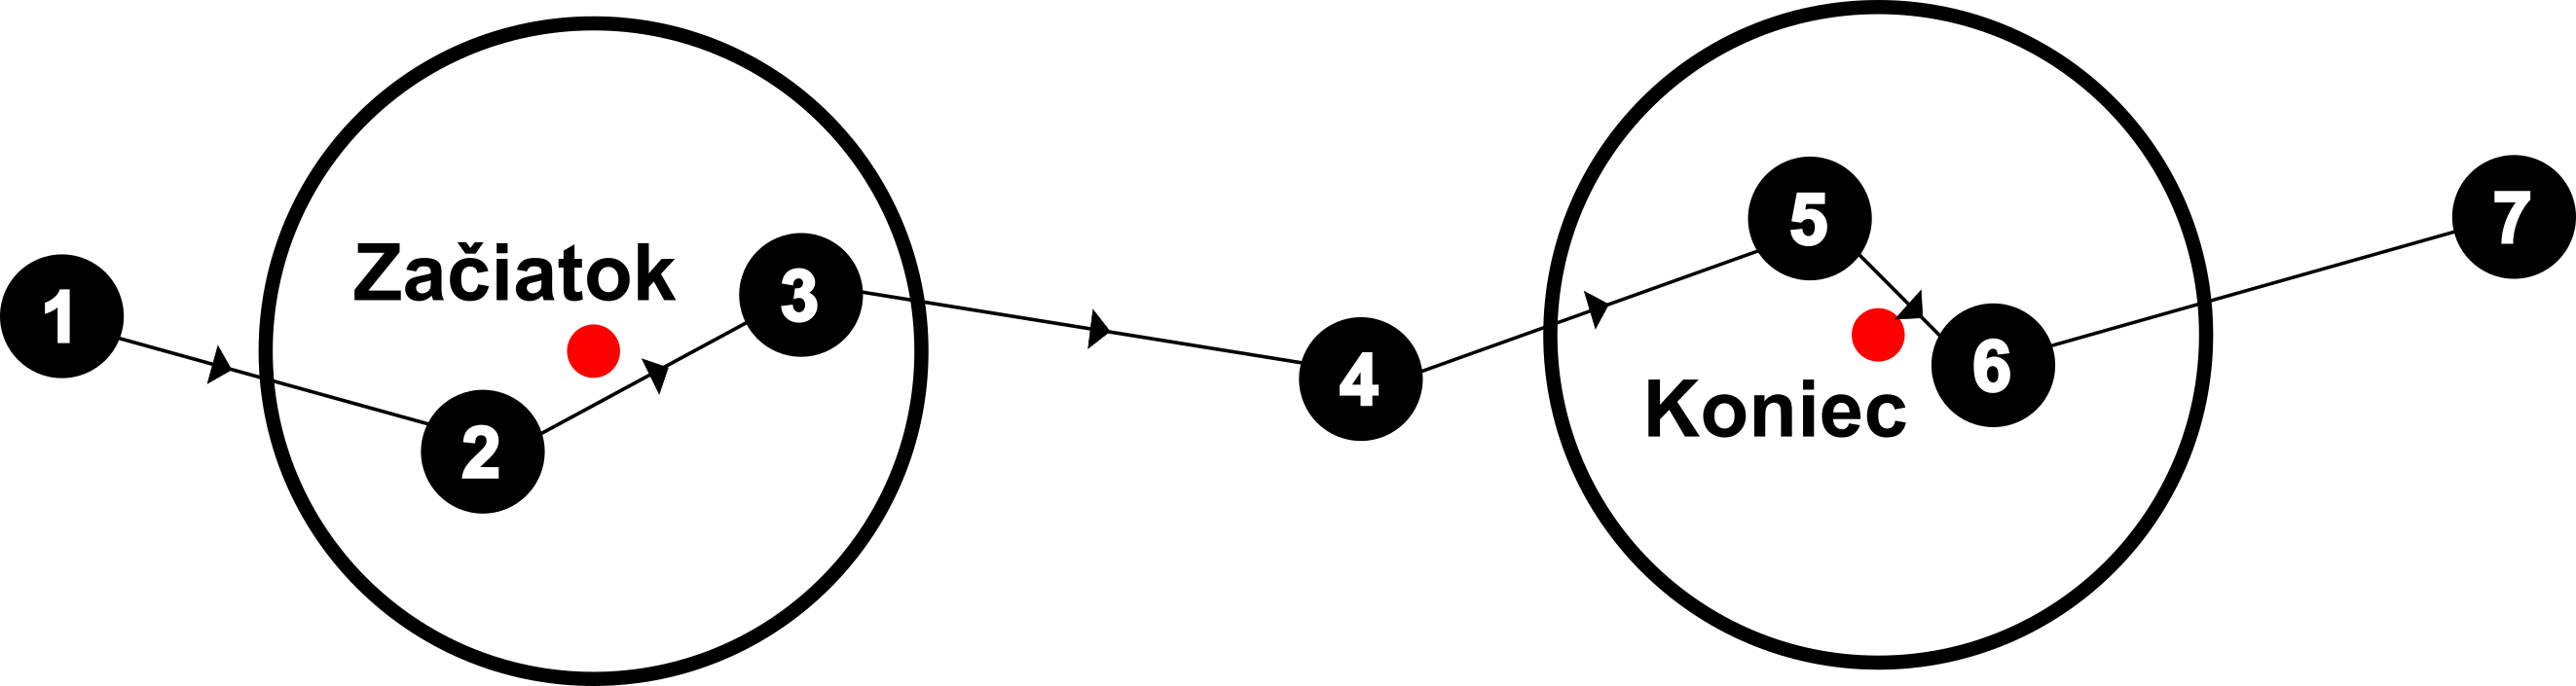
\includegraphics[width=0.7\textwidth]{images/circular-route}}
\caption[Hľadanie správnej začiatočnej/konečnej zastávky]{Hľadanie správnej začiatočnej/konečnej zastávky}
\label{fig:circularRoute}
\end{figure}

\section{Alternatívne optimálne cesty}
Pri hľadaní optimálnej cesty je potrebné zohľadniť, čo daný používateľ považuje za optimálne. Používateľ pri zadávaní vyhľadávacích parametrov nemusí poznať svoje preferencie alebo ich môže často meniť. Zadávanie preferencií pri každom vyhľadávaní nie je používateľsky prívetivé. Aby si napriek tomu používateľ mohol zvoliť cestu, ktorá najviac vyhovuje jeho potrebám, systém musí ponúknuť viac alternatívnych ciest. Tu sa dostávame k problému \textit{K} najkratších ciest.

Autori článku \cite{dissimilar}, poukazujú na to, že väčšina navigačných služieb neposkytuje používateľom viac ciest. A ak áno, využívajú taký algoritmus, ktorý poskytuje viacero alternatívnych ciest, ktoré sú podobné vo veľkej časti úsekov. Správny algoritmus by mal vybrať trasy s najmenšou spoločnou dĺžkou spomedzi tých, ktoré vyhovujú zadaným preferenciám. Autori článku predstavili vývoj heuristického algoritmu, ktorý efektívne vyhľadáva rôzne alternatívne cesty. Algoritmus je popísaný vývojovým diagramom na obrázku \ref{fig:flowchart}.

\begin{figure}[H]
\centerline{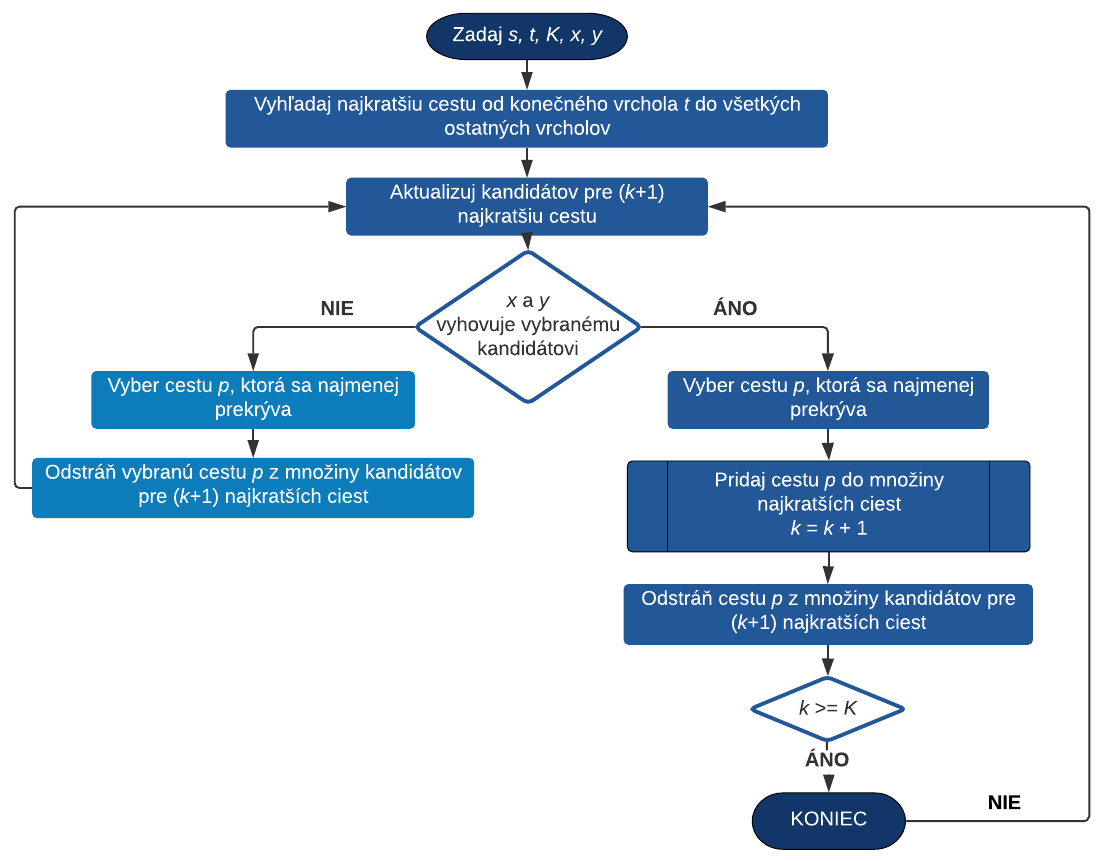
\includegraphics[width=1.0\textwidth]{images/flow-chart}}
\caption[Algoritmus K najkratších ciest - vývojový diagram]{Algoritmus K najkratších ciest - vývojový diagram}
\label{fig:flowchart}
\end{figure}

\section{RAPTOR algoritmus}
\label{sec:raptor}
Doteraz spomínané algoritmy riešia problém hľadania optimálnej cesty vo verejnej doprave ako grafový problém. Ako sme uviedli v predchádzajúcich sekciách, najčastejšie sa pre tento problém vytvorí model dopravnej siete pomocou grafu a na ňom sa spustí algoritmus hľadania najkratšej cesty. Týmto riešením však väčšinou dostávame menej optimálne výsledky za vysoké výpočtové časy.

Techniky, ktoré sa opierajú o grafové modely ťažko spracúvajú dynamickosť v systémoch verejnej dopravy, ako časté meškanie liniek, náhle zrušenie liniek, zmeny trás a podobne. Hoci algoritmy hľadania najkratšej cesty sú rýchle, práve vytvorenie modelu spôsobuje spomínané vysoké výpočtové časy.

Autori článku \cite{raptor} predstavujú RAPTOR – Round-bAsed Public Transit Optimal Router, ktorý dokáže byť oveľa rýchlejší použitím jednoduchých obmedzovacích pravidiel a paralelizmu. Keďže RAPTOR algoritmus nepotrebuje žiadny grafový model, dokáže fungovať rýchlo a dynamicky. Pre dve zadané zastávky vráti všetky optimálne cesty s minimálnym časom príchodu do konečnej zastávky a minimálnym počtom prestupov. Algoritmus beží v kolách a počíta časy príchodu prechádzaním jednotlivých trás.

Na rozdiel od grafových algoritmov, RAPTOR sa ľahko paralelizuje. Jednoducho rozdelí nezávislé linky medzi rôzne CPU jadrá. Existujú dve rozšírenia algoritmu a to McRAPTOR, ktorý zvláda riešiť viacero kritérií okrem času príchodu a počtu prestupov a rRAPTOR, ktorý vracia množinu ciest pre všetky odchody zo zastávky v danom časovom rozsahu. Bez potrebného pre-processingu a post-processingu dokáže spracovať aj kritérium preferovaných prestupných miest.

\subsection{Definície pojmov a premenných}

Definujeme cestovný poriadok ako $(\mathcal{S,T,R,F},\Pi)$, kde 
\begin{itemize}
\item $\Pi \subset \mathbb{N}_{0}$ je čas v sekundách, 
\item $\mathcal{S}$ je množina zastávok,
\item $\mathcal{T}$ je množina jázd, 
\item $\mathcal{R}$ je množina liniek a 
\item $\mathcal{F}$ je množina peších presunov.
\end{itemize}

Zastávka $p$ predstavuje miesto pre nastúpenie a vystúpenie z vozidla. Môže to byť aj platforma. Jazda $t$ reprezentuje postupnosť zastávok konkrétneho vozidla. Každá zastávka $p$ z jazdy $t$ má priradený čas odchodu $\tau_{dep}(t, p) \in \Pi$ a čas príchodu $\tau_{arr}(t, p) \in \Pi$. Každá linka z $\mathcal{R}$ pozostáva z jázd, ktoré majú rovnaké postupnosti zastávok. Pešie prechody z množiny $\mathcal{F}$ reprezentujú prestupy medzi zastávkami. Každý prestup pozostáva z dvoch zastávok $p_1$ a $p_2$ a času potrebného na presun medzi nimi $l(p_1, p_2)$. 

Výstupom z algoritmu je cesta $\mathcal{J}$, ktorá je definovaná postupnosťou jázd a peších prestupov. Cesta, ktorá obsahuje $k$ jázd, má presne $k-1$ prestupov. Majme začiatočnú zastávku $p_s$ a konečnú zastávku $p_t$ a čas odchodu $\tau$. Najzákladnejším kritériom, na ktoré algoritmus prihliada, je \textit{Earliest Arrival Problem}, ktorý hľadá cestu nezačínajucú skôr než $\tau$ v bode $p_s$ a do $p_t$ sa dostane čo najrýchlejšie. Ďalej chceme viacero alternatívnych ciest s tým, že žiadna z ciest nezačína skorej ako $\tau$ a cesty môžu obsahovať aj prestupy. 

\subsection{Základná verzia algoritmu}
\label{sub:raptor-basic}

Nech $p_s \in \mathcal{S}$ je začiatočný vrchol a $\tau \in \Pi$ je čas odchodu. Cieľom je vypočítať pre každé $k$ cestu do zastávky $p_t$ s minimálnym časom príchodu, ktorá je zložená z najviac $k$ jázd. Algoritmus beží v $k$ kolách. Kolo $k$ počíta najrýchlejšiu cestu do každej zastávky na $k-1$ prestupov. Niektoré zastávky nemusia byť dosiahnuteľné. Pri objasňovaní algoritmu bude počet kôl rovný $K$. Algoritmus pridelí každej zastávke $p$ postupnosť $(\tau_0(p), \tau_1(p), ..., \tau_K(p))$, kde $\tau_i(p)$ reprezentuje najskorší známy čas príchodu do zastávky $p$ na najviac $i$ jázd. 

Na začiatku sú všetky hodnoty vo všetkých postupnostiach pre každú zastávku inicializované na hodnotu $\infty$. Nastavíme $\tau_0(p_s) = \tau$. Dodržuje sa invariant: na začiatku kola $k$ je prvých $k$ hodnôt v postupnosti $\tau(p)$ správnych a ostatné hodnoty majú hodnotu $\infty$. Cieľom kola $k$ je vypočítať $\tau_k(p)$. Tento výpočet sa vykonáva v troch krokoch. 
 
V prvom kroku kola $k$ (ak $k \neq 0$) sa nastaví pre všetky zastávky $p$ hodnota $\tau_k(p) = \tau_{k-1}(p)$. Týmto nastavíme horné ohraničenie na najskorší príchod do zastávky $p$ na najviac $k$ jázd.

Druhé kolo spracuje práve raz každú linku $r$. Nech $\mathcal{T}(r) = (t_0, t_1, ..., t_{|\tau(r)|-1})$ je postupnosť jázd pre linku $r$ zoradená od najskôr začínajúcej po poslednú jazdu. Nech $et(r, p_i)$ je najskoršia jazda linky $r$, na ktorú je možné nastúpiť na zastávke $p_i$. Táto hodnota nemusí byť vždy definovaná. Pri spracovaní linky $r$ navštevujeme jej zastávky a hľadáme takú zastávku $p$, kde je hodnota $et(r, p_i)$ definovaná. Označme prislúchajúcu jazdu ako aktuálnu jazdu pre $k$. Ďalej prechádzame linku a pre každú zastávku $p_j$ aktualizujeme $\tau_k(p_j)$ použitím tejto jazdy. Aby sme vedeli spätne určiť výslednú cestu, nastavíme smerník na zastávku, na ktorej sme nastúpili na jazdu $t$. Navyše bude potrebné aktualizovať aktuálnu jazdu pre $k$. Na každej zo zastávok $p_i$ na linke $r$ môžeme stihnúť skoršiu jazdu, pretože sme v predchádzajúcich kolách mohli nájsť rýchlejšiu cestu do $p_i$. Je potrebné skontrolovať či $\tau_{k-1}(p_i) < \tau_{arr}(t, p_i)$ a aktualizovať $t$ prepočítané $et(r, p_i)$.

V treťom kroku zvažujeme pešie presuny. Zo zastávky $p_i$ sa môžeme dostať do niektorých zastávok peším presunom. Treba overiť, či týmto presunom nedosiahneme skorší čas príchodu do niektorej zo zastávok. Pre každý peší presun $(p_i, p_j) \in \mathcal{F}$ nastaví $\tau_k(p_j) = min\{\tau_k(p_j), \tau_k(p_i) + l(p_i, p_j)\}$. 

Algoritmus sa končí, keď po kole $k$ nebola vylepšená žiadna z hodnôt $\tau_k(p_i)$. 

Najhorší odhad časovej zložitosti algoritmu je lineárny, konkrétne $\mathcal{O}(K(\sum_{r \in \mathcal{R}} |r| + |\mathcal{T}| + |\mathcal{F}|)$, kde $K$ je počet kôl, pričom v každom kole $k$ prechádzame každú linku $r$ najviac jeden krát. Keďže $|r|$ je počet zastávok, spolu prechádzame $\sum_{r \in \mathcal{R}} |r|$ zastávok. Pri počítaní $et(r, p_i)$, prechádzame každú jazdu $t$ linky $r$ najviac jeden krát. 

\subsection{Optimalizácie algoritmu}
\label{sub:raptor-optimalisation}
Pri hľadaní najkratšej cesty je prechádzanie všetkých liniek v každom kole zbytočné. V niektorých prípadoch neexistuje možnosť prestúpiť medzi dvoma linkami, takže niektoré z liniek sú nedosiahnuteľné. Majme linku $r$ a majme zastávku $p$ v $r$, ktorej posledné vylepšenie času príchodu bolo v kole $k' < k-1$. Linka $r$ bola opäť navštívená v kole $k'+1 < k$, ale žiadnej z jej zastávok sa nevylepšil čas príchodu. Nie je dôvod prechádzať linku znovu, ak aspoň jedna z jej zastávok nebola vylepšená. 

Na implementáciu tejto optimalizácie postačí, ak si v kole $k-1$ označíme tie zastávky, pre ktoré bol v tomto kole vylepšený čas $\tau_{k-1}(p_i)$. Na začiatku kola $k$ prejdeme cez všetky tieto zastávky, označíme ich a nájdeme všetky linky, ktorým zastávky prislúchajú. Označené zastávky sú potenciálne miesta na prestup medzi linkami v kole $k$. Stačí nám dokonca prechádzať linku od prvej označenej zastávky v linke. Pridáme linky do pola $Q$ a zapamätáme si jej prvú označenú zastávku. 

Príklad môžeme vidieť na obrázku \ref{fig:raptor-optimal}. Algoritmus hľadá cestu zo zastávky $p_s$ do zastávky $p_t$. V prvom kole spracuje linku $r_1$, v druhom kole linky $r_2$ a $r_3$ a v treťom kole linku $r_4$. Iterovanie linky začína v prvej označenej zastávke linky (žltá farba). Zastávky označené bielou farbou nebudú po optimalizácii spracované v žiadnom kole. 

\begin{figure}[H]
\centerline{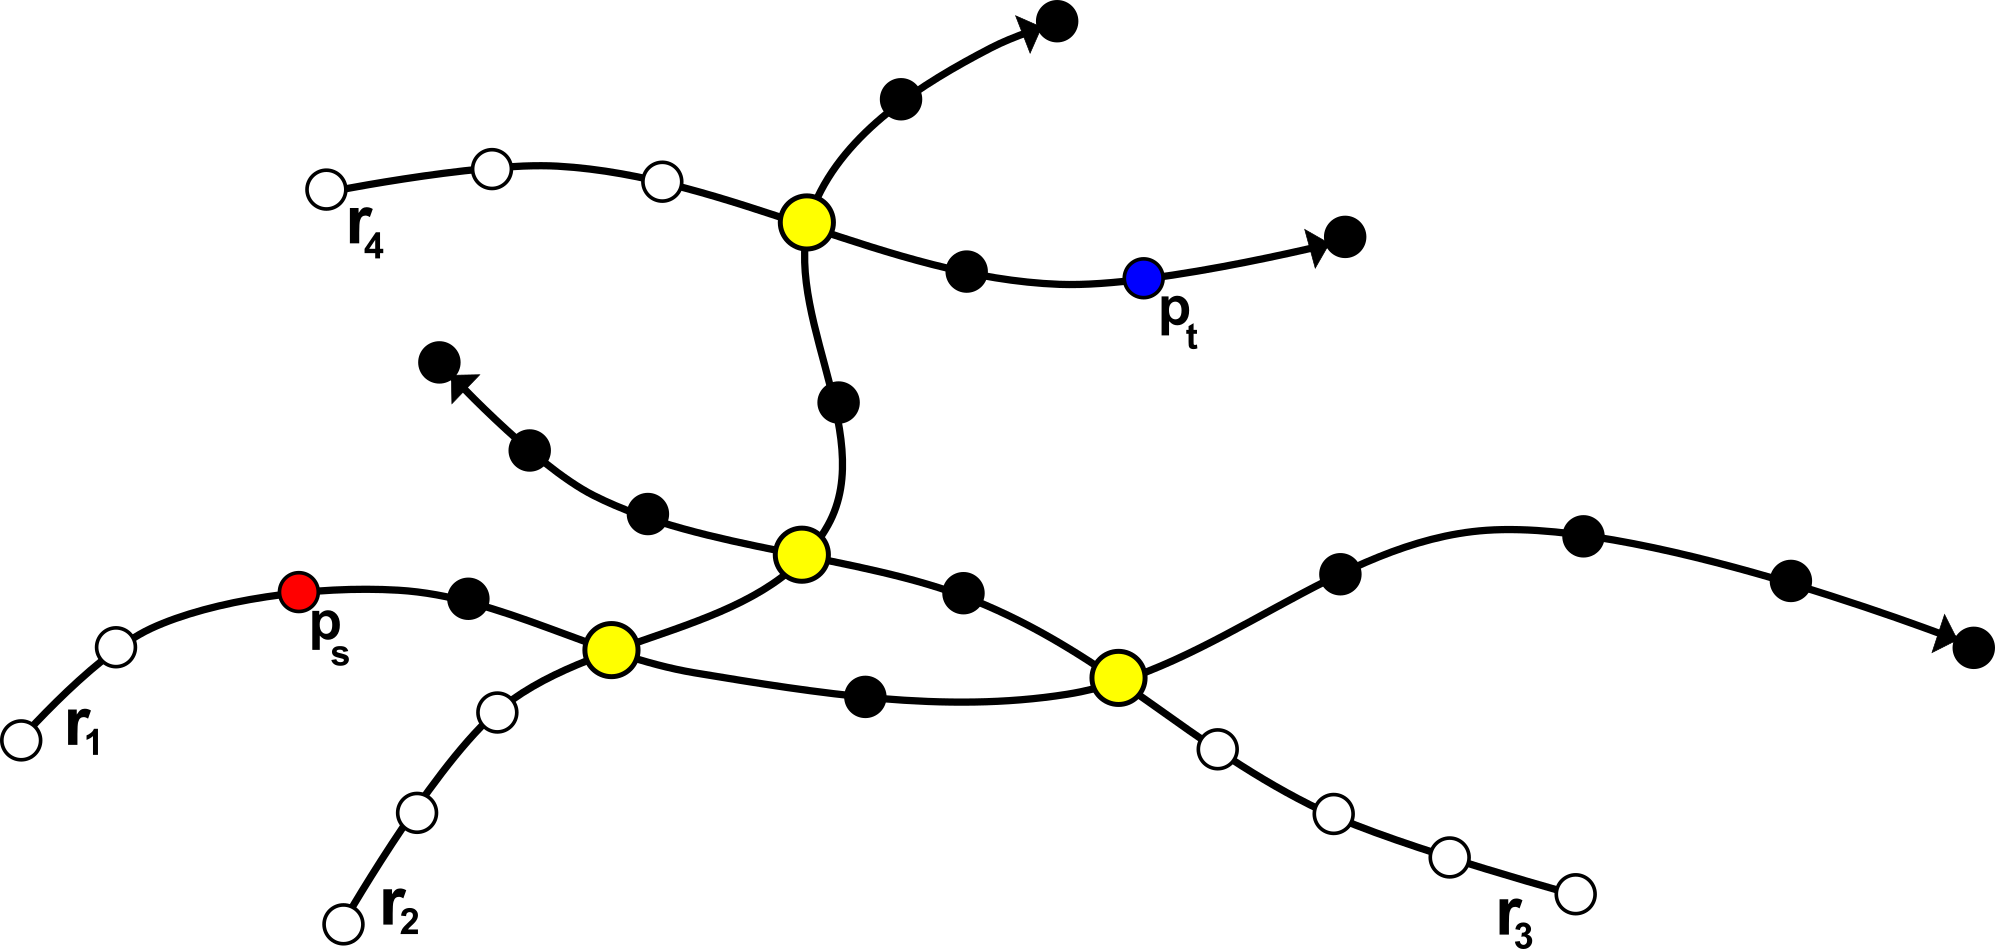
\includegraphics[width=0.8\textwidth]{images/raptor-optimal}}
\caption[RAPTOR - Optimalizácia prechádzania liniek]{RAPTOR - Optimalizácia prechádzania liniek}
\label{fig:raptor-optimal}
\end{figure}

Ďalšou optimalizačnou technikou je \textit{local prunning}. Pre každú zastávku $p_i$ si udržujeme hodnotu $\tau^*(p_i)$, ktorá reprezentuje najskorší známy čas príchodu na zastávku $p_i$. Vylepšením je, že zastávku označíme len v prípade, že čas príchodu v kole $k$ je menší ako predchádzajúca hodnota $\tau^*(p_i)$. 

RAPTOR algoritmus hľadá cestu zo začiatočnej zastávky do všetkých zastávok, hoci chceme nájsť cestu do konkrétnej konečnej zastávky. \textit{Target prunning} obmedzí hľadanie ciest do všetkých vrcholov na hľadanie jednej cesty. Dosiahneme to, ak v kole $k$ nebudeme označovať zastávky $p_i$, pre ktoré platí $\tau^*(p_i) > \tau^*(p_t)$.   

\subsection{rRAPTOR}
\label{sub:rraptor}
rRAPTOR je rozšírenie RAPTOR algoritmu, ktoré nám vráti množinu najkratších ciest pre všetky odchody zo zastávky v danom časovom rozsahu. 

Nech $\Delta \subseteq \Pi$ je časový úsek. Najskôr vložíme do množiny $\Psi$ časy odchodov jázd začínajúcich na danej zastávke, ktoré patria do časového úseku $\Delta$. Pre každý čas odchodu $\tau$ z $\Psi$ spustíme RAPTOR algoritmus nezávisle. Znamená to, že hodnota $\tau_k(p)$ bude existovať pre každý čas odchodu $\tau$, zastávku $p$ a kolo $k$. Nemusí platiť, že všetky nájdené cesty budú optimálne. Na porovnanie ciest využijeme pravidlo dominancie ciest: cesta $\mathcal{J}_1$ dominuje nad cestou $\mathcal{J}_2$, ak platí:

$\tau_{dep}(\mathcal{J}_1) \geq \tau_{dep}(\mathcal{J}_2)$ a $\tau_{arr}(\mathcal{J}_1) \leq \tau_{arr}(\mathcal{J}_2)$. 

Aby sme mohli použiť toto pravidlo, zoradíme časy v množine $\Psi$ od najneskoršieho po najskorší čas. Pri iterovaní nebudeme prepisovať hodnotu $\tau_k(p)$ medzi kolami, ale nastavíme vždy na začiatku kola pre všetky zastávky $p$ $\tau_k(p) = \tau_{k-1}(p)$, kde je $\tau_{k-1}(p)$ lepšie ako $\tau_k(p)$. Pri tomto rozšírení algorimu nemôžeme použiť \textit{local prunning}, keďže nechceme, aby sa hodnota $\tau^*(p)$ porovnávala s ďalším spustením algoritmu pre skoršie časy z množiny $\Psi$. 


\subsection{Paralelizácia}
Ako sme si mohli všimnúť, linky sú individuálne a nie je potrebné ich iterovať v špecifickom poradí. Ak máme k dispozícii viac CPU jadier, každé z nich môže spracovávať inú podmnonžinu liniek. Nákladné môže byť zamedzenie prístupu do spoločného miesta v pamäti $(\tau_k(p))$. Autori navrhli 2 prístupy na riešenie paralelizácie bez využitia zámkov. Jeden prístup počíta s tým, že hardvér zaisťuje atomické zapisovanie do pamäte a druhý sa zaobíde aj bez tejto možnosti. 

\subsection{Dátová štruktúra}
\label{subsec:structure}
Autori článku navrhli aj štruktúru, ktorá je vhodná pre RAPTOR algoritmus. Linky, jazdy a zastávky indexujeme od $0$. Potrebujeme pole liniek \textit{Routes}, ktoré si pre každú linku $r_i$ uchováva informáciu o počte zastávok na linke $r_i$ a smerník na pole \textit{RouteStops}, ktorý označuje začiatok postupnosti zastávok na linke $r_i$. Podobne aj pre jazdy si linka $r_i$ uchováva smerník, ktorý ukazuje na začiatok bloku v poli \textit{StopTimes}. Jeden blok v poli \textit{StopTimes} obsahuje všetky jazdy prislúchajúce linke $r_i$ zoradené podľa času odchodu z prvej zastávky. Každú jazdu reprezentuje postupnosť časov (čas príchodu a čas odchodu). Štruktúra ja zobrazená na obrázku \ref{fig:raptor-structure}. 

\begin{figure}[H]
\centerline{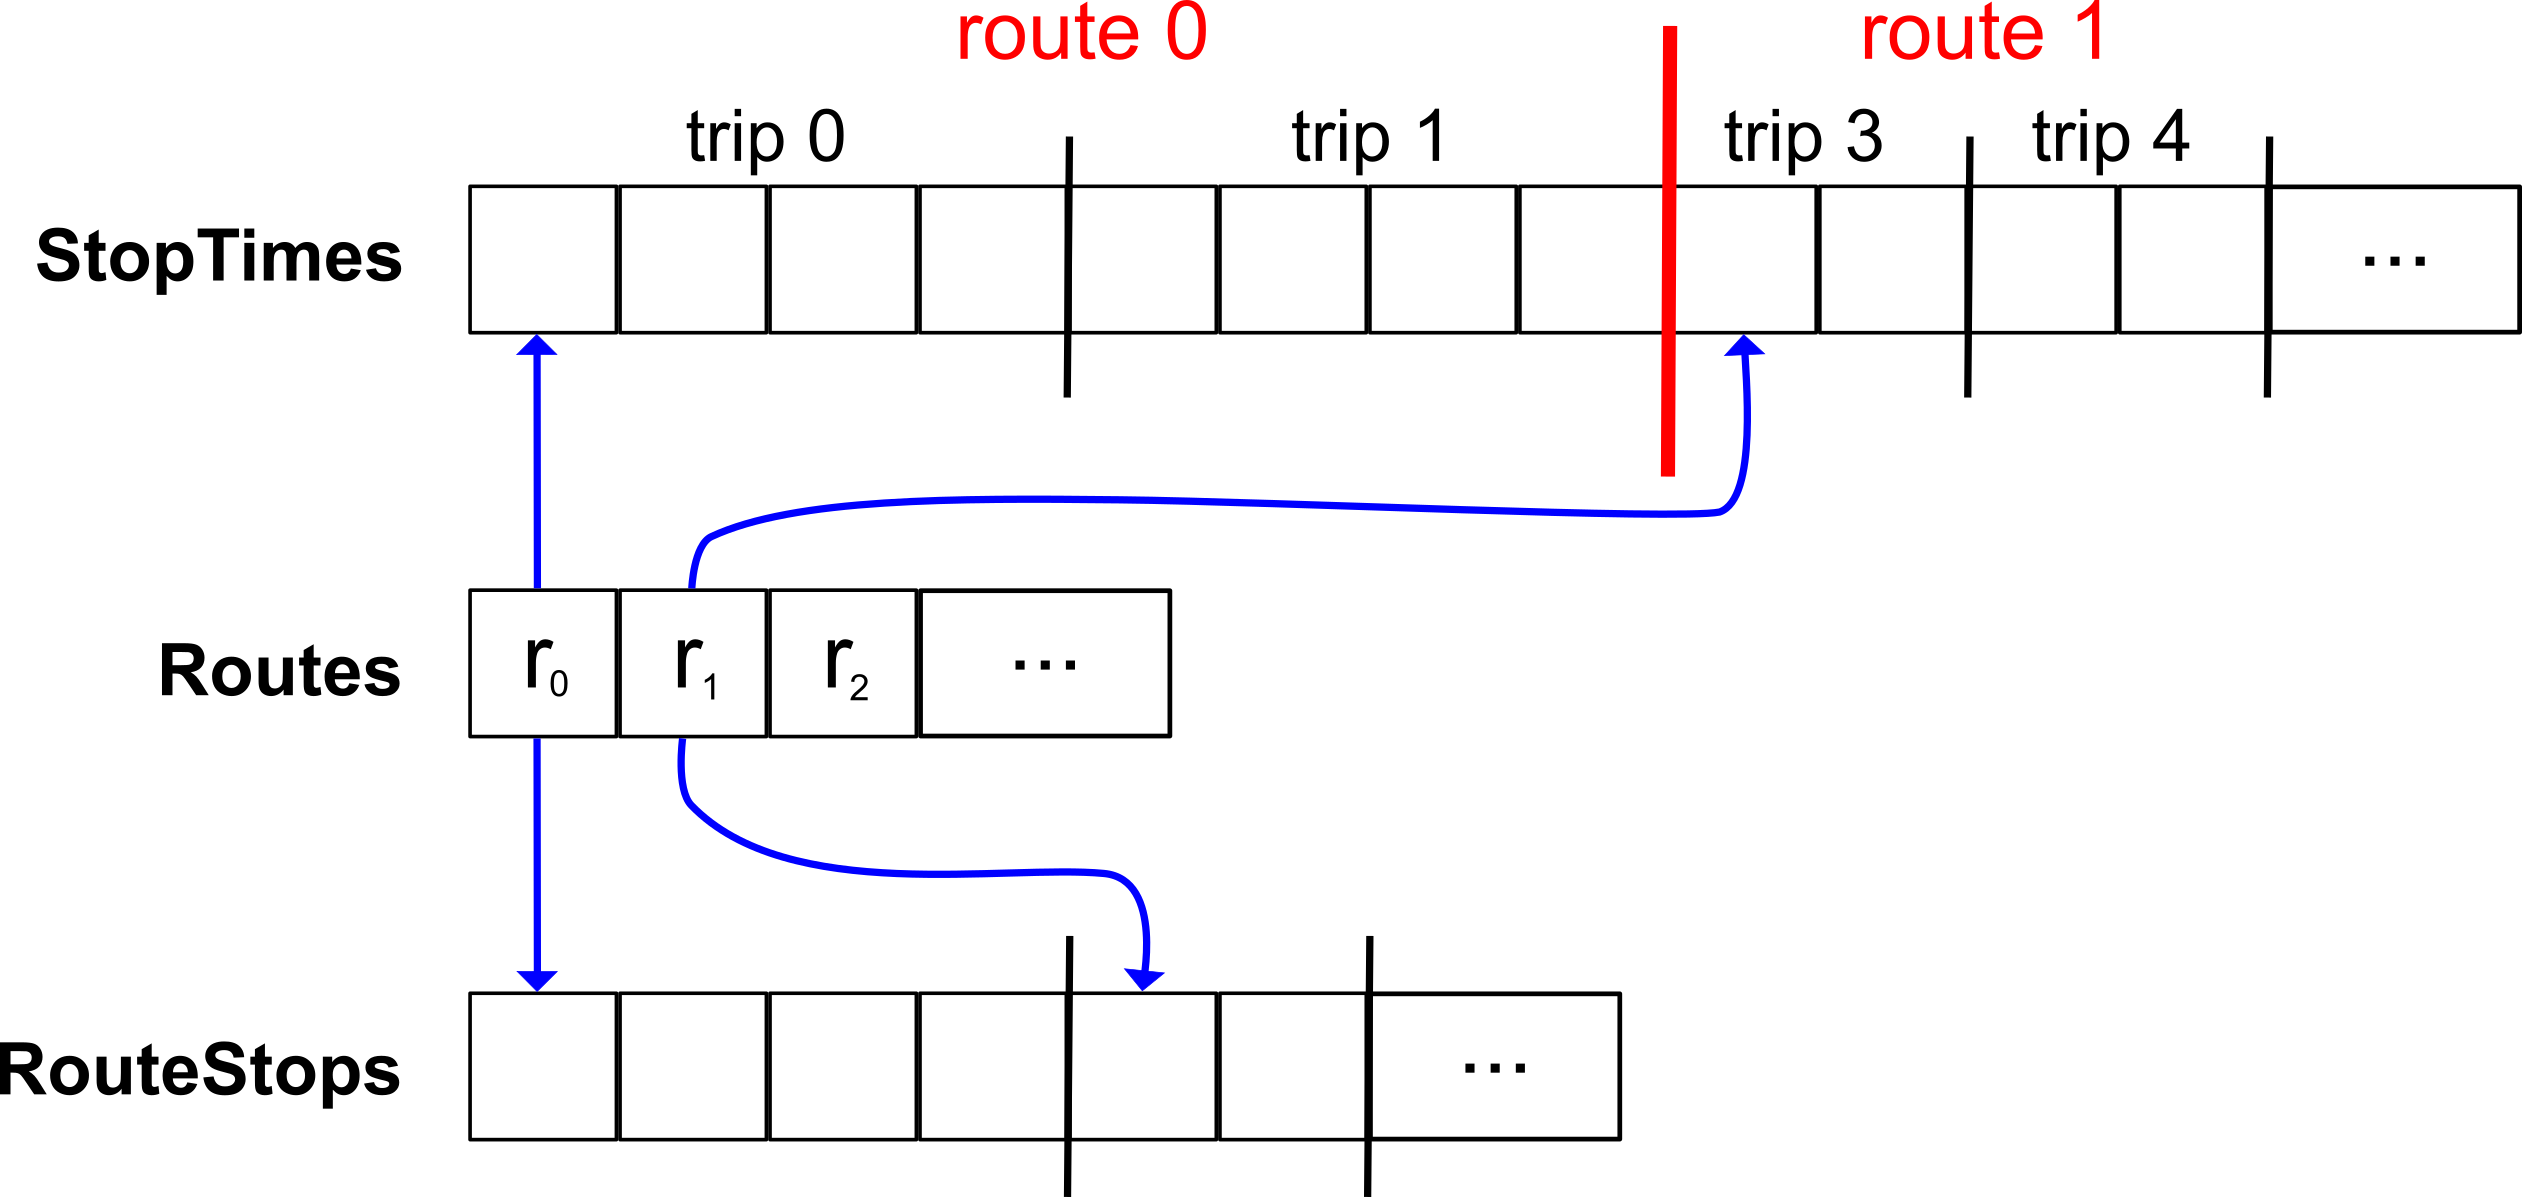
\includegraphics[width=0.7\textwidth]{images/raptor-structure}}
\caption[RAPTOR - Dátová štruktúra]{RAPTOR - Dátová štruktúra}
\label{fig:raptor-structure}
\end{figure}

V algoritme často potrebujeme iterovať cez zastávky linky $r_i$. Na to nám slúži pole \textit{RouteStops}. Ak potrebujeme získať najskorší čas odchodu zo zastávky $p$ po čase $\tau$, spôsob akým je pole \textit{StopTimes} utriedené nám zabezpečí, že čas tejto operácie bude konštantný.
Pri kontrolovaní, či sa v predchádzajúcej jazde nezlepšil čas odchodu niektorej zo zastávok, potrebujeme preskočiť na predchádzajúcu jazdu v poli \textit{StopTimes}. Na urýchlenie tejto operácie máme uloženú informáciu o počte zastávok pre linku $r_i$.

Takto navrhnutá štruktúra nie je pre algoritmus dostatočná. Na zohľadnenie prestupov potrebujeme ďalšie štruktúry a to pole \textit{Stops}, ktoré obsahuje všetky zastávky. Ďalej pole \textit{StopRoutes}, ktoré má pre každú zastávku priradené linky, ktoré na nej zastavujú. Pole \textit{Transfers}, ktoré obsahuje informácie o peších prechodoch medzi zastávkami. Pre každú zastávku je priradená dvojica: cieľová zastávka a čas potrebný na peší presun na túto zastávku. Náčrt doplňujúcej dátovej štruktúry je na obrázku \ref{fig:raptor-structure2}.

\begin{figure}[H]
\centerline{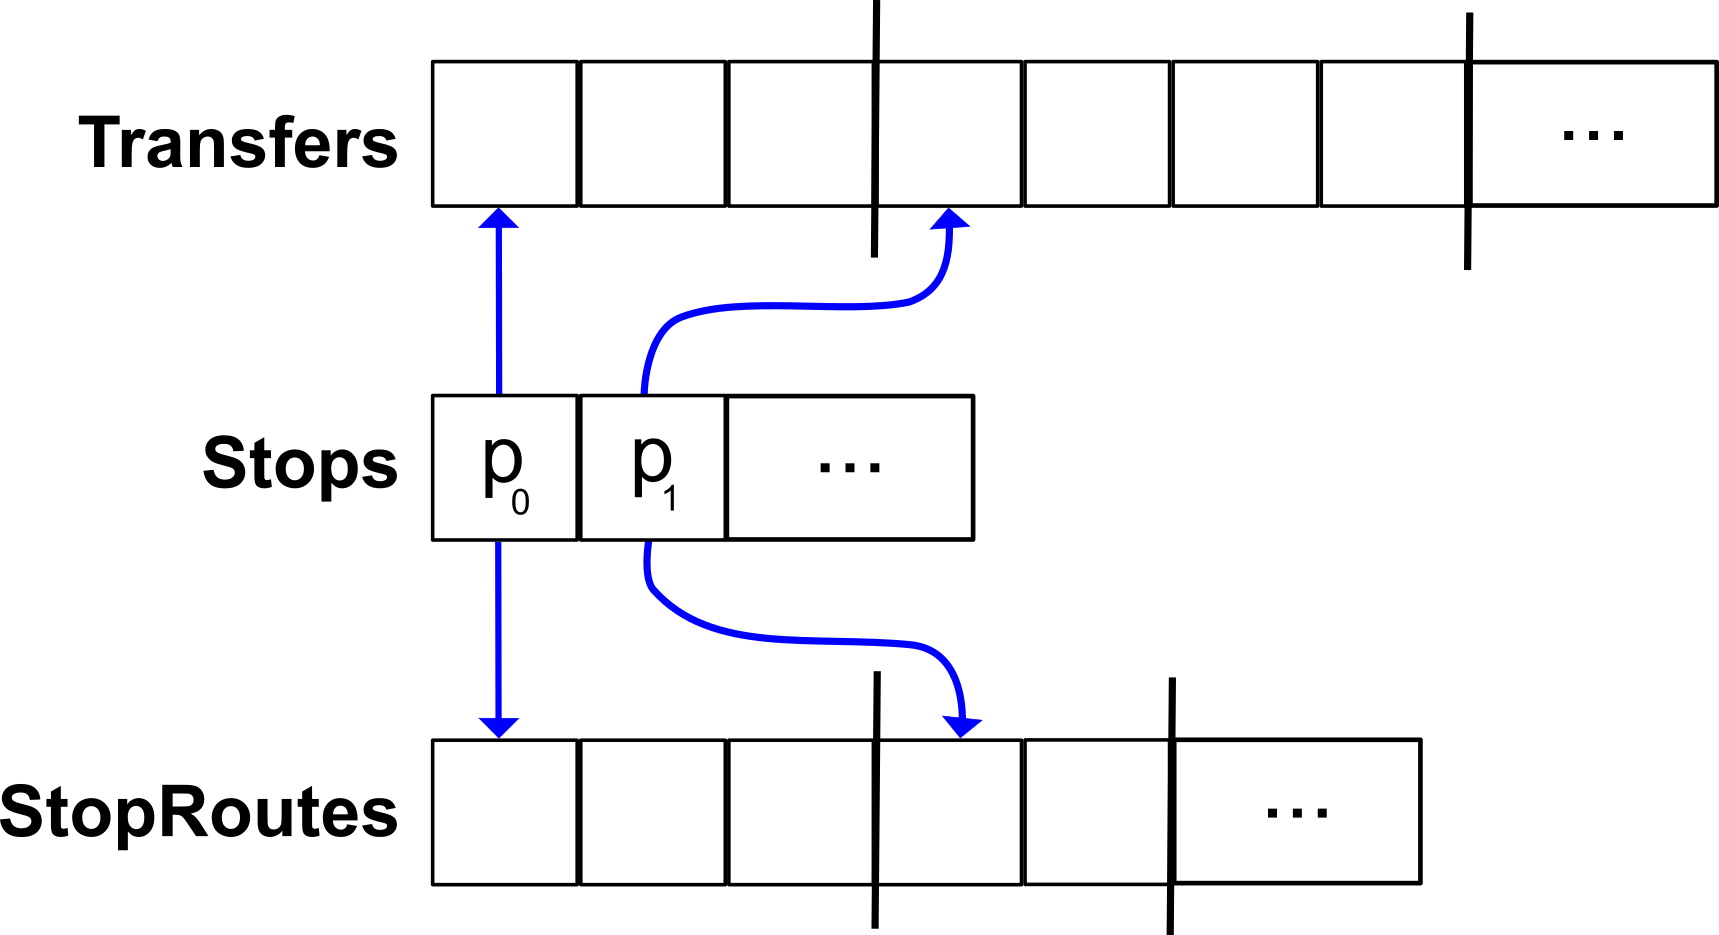
\includegraphics[width=0.5\textwidth]{images/raptor-structure2}}
\caption[RAPTOR - Dátová štruktúra na zohľadnenie prestupov]{RAPTOR - Dátová štruktúra na zohľadnenie prestupov}
\label{fig:raptor-structure2}
\end{figure}

\subsection{Vylepšený RAPTOR algoritmus}
\label{sec:raptor-improved}
Za výslednú cestu považoval RAPTOR algoritmus tú cestu, ktorá stojí najmenej času nezávisle od toho, koľko prestupov vyžaduje. Keďže cestujúci v skutočnosti nepreferujú cesty s veľkým počtom prestupov, je potrebné zaviesť do algoritmu ich penalizáciu. Ako sme už spomínali v predchádzajúcich sekciách, v prípade verejnej dopravy, ktorá má viacero módov, je nutné vyhľadať a ponúknuť cestujúcemu viacero alternatívnych ciest. Pôvodný RAPTOR algoritmus vracia len jednu najkratšiu cestu. 

V článku \cite{improvedRaptor} bol navrhnutý vylepšený RAPTOR algoritmus, ktorý má v sebe zapracovanú penalizáciu prestupov, korekčný faktor peších prestupov a vracia $k$ alternatívnych ciest. Cesty vypočítané vylepšeným algoritmom sa oveľa viac podobajú cestám, ktoré si v realite cestujúci vyberajú.

V tomto článku nám pribudlo označenie $k$-tej najkratšej cesty. Kedže písmenom $k$ sme doteraz označovali kolá, budeme hľadať $m$-tú najkratšiu cestu. Taktiež pribudli nové označenia a premenné, ktoré sú uvedené v tabuľke \ref{table:raptor-variables}.

\begin{table}[H]
\begin{tabular}{|l|l|}
\hline
\rowcolor[HTML]{C0C0C0} 
\textbf{Premenná} & \textbf{Popis} \\ \hline
$t_r$             & jazda $t$ linky $r$          \\ \hline
$Tr_c$             & penalizácia prestupu typu $c$          \\ \hline
$l(p, p_i)$       & čas pešieho prestupu zo zastávky $p$ do zastávky $p_i$ \\ \hline
$\tau_k(p)$			& najskorší známy čas príchodu na zastávku $p$ v $k$ kolách \\ \hline
$\tau_k(t, p)$    & najskorší známy čas príchodu na zastácku $p$ použitím jazdy $t$ v $k$ kolách \\ \hline
$\mathcal{J}_k(p)$ & množina ciest, ktorými sa viam dostať na zastávku $p$ v $k$ kolách \\ \hline
$\mathcal{J}_{k,m}(p)$ & $m$-tá najskoršia cesta, ktorou sa viem dostať na zastávku $p$ v $k$ kolách \\ \hline
$\mathcal{J}_k(p, p_i)$ & cesta zo zastávky $p$ do zastávky $p_i$ v $k$ kolách \\ \hline
\end{tabular}
\caption{Tabuľka premenných pre vylepšený RAPTOR algoritmus}
\label{table:raptor-variables}
\end{table}

\subsubsection{Penalizácia prestupov}
Penalizácia prestupov je pojem zahŕňajúci časové a nečasové prvky prestupu. Medzi časové prvky patrí čakanie na prestupný spoj a čas potrebný na peší presun. Nečasovými prvkami môže byť pohodlie a komplikovanosť prestupu, ktoré závisia najmä od toho, či prestupujeme medzi rovnakými módmi alebo sa módy líšia. 

Autori článku definujú dva druhy prestupov: horizontálny a vertikálny. Napríklad prestup medzi autobusmi je horizontálny, ale pri prestupe z autobusu na metro je potrebné použiť schody a preto sa jedná o vertikálny prestup. Podľa druhu prestupu $c$ aplikujeme penalizáciu prestupu $Tr_c$. Pri implementácii si potrebujeme pamätať predchádzajúci mód jazdy, ktorým cestujúci prišiel na zastávku, na ktorej bude prestupovať.

Čo sa týka času potrebného na peší presun medzi jednotlivými zastávkami, priemerná rýchlosť kráčania dospelého človeka bola určená na $1.2 m/s$. Väčšinou sa predpokladá, že dĺžka prestupu je Euklidovská vzdialenosť od počiatočnej zastávky po cieľovú. Tento odhad ale nie je vyhovujúci, pretože vo väčšine prípadov je trasa prestupu dlhšia ako vzdušná čiara medzi zastávkami. Navrhli preto použiť Manhattanovskú vzdialenosť. Keď je vzdialenosť vzdušnou čiarou rovná 1, Manhattanovská vzdialenosť má hodnotu $\sqrt{2}$.

\subsubsection{Hľadanie viacerých ciest}
Vylepšený algoritmus hľadá $M$ najkratších ciest. Je potrebné zabrániť tomu, aby v rámci $m$-nájdených ciest boli podobné cesty. Autori navrhli 2 pravidlá, použitím ktorých zabránia výskytu podobných ciest vo výsledných $M$ cestách.

Prvým pravidlom je, že jazda $t$ linky $r$ by sa už znova nemala vyhľadať zo zastávky, na ktorej cestujúci vystúpi. Príklad je na obrázku \ref{fig:similar-paths}(a). Červená cesta vedie priamo zo začiatočnej zastávky $S$ do konečnej zastávky $T$ a modrá cesta obsahuje navyše prestup na zastávke $A$. Časy príchodu týchto dvoch ciest sa líšia a preto by sa cesty vyhodnotili ako rôzne. Týmto zabránime tomu, aby červená a modrá cesta boli vybrané súčasne.

Druhé pravidlo považuje cesty za podobné, ak je postupnosť zastávok v oboch cestách rovnaká. Na obrázku \ref{fig:similar-paths}(b) môžeme vidieť, že cesty sa líšia v mieste prestupu a tým pádom aj v čase príchodu do cieľovej zastávky. Preto by tieto cesty boli vyhodnotené ako rozdielne. Po aplikovaní pravidla budú vyhodnotené ako podobné. 
V $\mathcal{J}_k(p)$ sú uložené cesty, ktorými sme sa dostali na zastávku $p$ v kole $k$. Ak prídeme na zastávku $p$ v čase $\tau_k(p)$, porovnáme časy príchodov už existujúcich ciest z množiny $\mathcal{J}_k(p)$ a len cesta s minimálnym časom príchodu bude aktualizovaná.

\begin{figure}[H]
\centerline{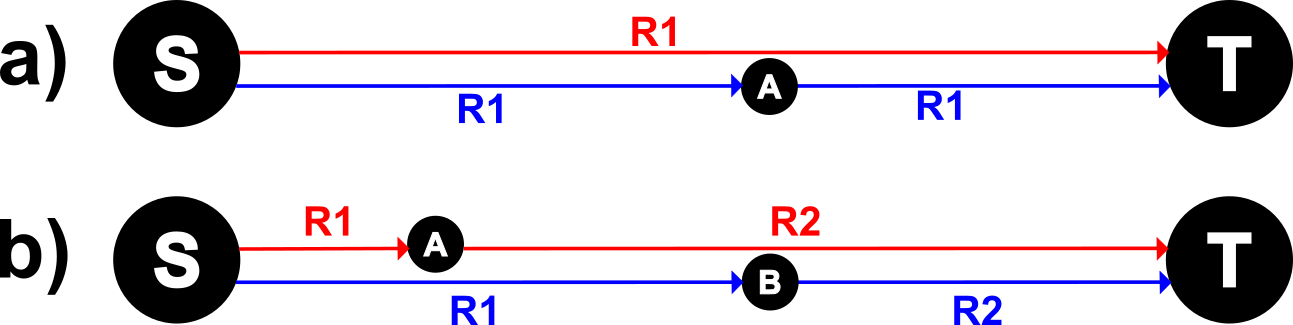
\includegraphics[width=0.7\textwidth]{images/similar-paths}}
\caption[RAPTOR - podobné cesty]{RAPTOR - podobné cesty}
\label{fig:similar-paths}
\end{figure}

Ďalej je popísaný algoritmus \ref{alg:1}, ktorý zhodnotí, či je cesta $\mathcal{J}_k(p, p_i)$ podobná ako niektorá z ciest zaznamenaných v množine $\mathcal{J}_k(p_i)$.

\begin{algorithm}
\caption{Algoritmus na zistenie podobných ciest}\label{alg:1}
 \hspace*{\algorithmicindent} \textbf{Input: $\mathcal{J}_k(p_i)$, $t_r$, $\mathcal{J}_k(p, p_i)$} \\
 \hspace*{\algorithmicindent} \textbf{Output: true or false} 
\begin{algorithmic}[1]
\ForEach{$\mathcal{J}_{k,m}(p_i) \in \mathcal{J}_k(p_i)$}
\If {last $t$ of $\mathcal{J}_{k,m}(p_i) = t_r$} \Return false
\ElsIf { $\mathcal{J}_k(p, p_i) = \mathcal{J}_{k,m}(p_i)$} \Return false
\Else {} \Return true
\EndIf
\EndFor
\end{algorithmic}
\end{algorithm}

\subsubsection{Zhrnutie vylepšeného RAPTOR algoritmu}
Algoritmus nám vráti $M$ najskorších ciest, ktoré vedú na zastávku $p_t$. Vstupom pre algoritmus je čas odchodu $\tau$, začiatočná zastávka $p_s$ a konečná zastávka $p_t$. Začíname v kole $m=0$. Pre každú zastávku $p$ nastavíme hodnotu $\tau_k(p)=\infty$, okrem začiatočnej zastávky $p_s$. Tá bude mať hodnotu $\tau_k(p_s)=\tau$ a bude označená.
\\
\\
\textbf{KROK 1:} Ak nie sme v kole $0$, pre každú zastávku $p$ nastavíme $\tau_k(p) = \tau_{k-1}(p)$ a $\mathcal{J}_k(p)=\mathcal{J}_{k-1}(p)$.\\
\textbf{KROK 2:} Pre každú zastávku $p$ označenú v kole $k-1$ hľadáme všetky zastávky $p_i$, na ktoré sa vieme dostať peším presunom zo zastávky $p$. Ak $\tau_k(t, p)$ cesty $\mathcal{J}_k(p, p_i)$ je skôr ako $\tau_k(p_i)$, tak do $\tau_k(p_i)$ vložíme hodnotu $\tau_k(t, p)$ a označíme zastávku $p_i$. Ak počet ciest v množine $\mathcal{J}_k(p_i) < K$, pridaj cestu $\mathcal{J}_k(p, p_i)$ do tejto množiny. Ak je veľkosť množiny rovnaká ako $K$, nahraď cestu $\mathcal{J}_{k,m}(p_i)$ cestou $\mathcal{J}_k(p, p_i)$ a označ zastávku $p_i$. Ak nastane nejaká zmena v množine $\mathcal{J}_k(p_i)$, zotrieď ju podľa času príchodu do zastávky $p_i$. \\
\textbf{KROK 3:} Pre každú označenú zastávku $p$, vložíme všetky dvojice $(r, p)$ do poľa $Q$, pričom platí, že linka $r$ obsluhuje zastávku $p$.\\
\textbf{KROK 4:} Pre každú dvojicu $(r, p)$ hľadáme jazdu $t_r$, ktorá príde na zastávku $p$ po čase $\tau_k(p) + Tr_c$.\\
\textbf{KROK 5:} Ak je posledná linka v množine $\mathcal{J}_{k,m}(p)$ identická s linkou $r$, preskoč KROK 6 a KROK 7.\\
\textbf{KROK 6:} Hľadaj jazdu $t_r$ linky $r$ a pre každú zastávku $p_i$, ktorá patrí tejto linke over, či existuje podobná cesta ceste $\mathcal{J}_k(p, p_i)$. Ak už podobná cesta existuje, pokračuj KROKOM 7. Inak, ak počet ciest v $\mathcal{J}_k(p_i) < K$, pridaj cestu $\mathcal{J}_k(p, p_i)$ do tejto množiny. Ak je veľkosť množiny rovnaká ako $K$, porovnaj čas $\tau_k(p_i)$ cesty $\mathcal{J}_{k,m}(p_i)$ s časom $\tau_k(t, p)$ cesty $\mathcal{J}_k(p, p_i)$. Ak je čas $\tau_k(t,p)$ menší, nahraď $\mathcal{J}_{k,m}(p_i)$ cestou $\mathcal{J}_k(p, p_i)$ a označ zastávku $p_i$.  Ak nastane nejaká zmena v množine $\mathcal{J}_k(p_i)$, zotrieď ju podľa času príchodu do zastávky $p_i$. \\
\textbf{KROK 7:} Nájdi cestu, ktorá má rovnakú postupnosť liniek akú má $\mathcal{J}_k(p, p_i)$ a ak platí $\tau_k(t, p)$ cesty $\mathcal{J}_k(p, p_i)$ < $\tau_k(p_i)$ cesty $\mathcal{J}_{k,m}(p_i)$, tak aktualizuj $\tau_k(p)$, označ zastávku $p_i$ a zotrieď množinu $\mathcal{J}_k(p_i)$\\
\textbf{KROK 8:} Ak existuje zastávka, ktorá má hodnotu $\tau_k(p)$ aktualizovanú v kole $k$, pokračuj v algoritme znovu od KROKU 1. Inak ukonči proces.

\section{Podobné existujúce systémy}
\label{sec:applications}
V tejto sekcii popíšeme niektoré existujúce mobilné aplikácie, ktoré umožňujú vyhľadávanie spojov v Bratislavskej mestskej hromadnej doprave. Z používania aplikácie nevieme zistiť, aký algoritmus používajú na vyhľadávanie spojení a v akých dátových štruktúrach udržujú dáta. Vieme však porovnať, aké funkcionality ponúkajú používateľom a zhodnotiť, čo nám chýba alebo prekáža pri používaní týchto aplikácii.

\subsection{Imhd.sk}
Mobilná aplikácia Imhd.sk ponúka vyhľadávanie MHD spojení v Bratislave a v Košiciach. Pri prvom spustení aplikácia sťahuje databázu cestovných poriadkov do úložiska zariadenia. Aplikácia funguje aj v offline režime, kedy používa cestovné poriadky, ktoré boli naposledy stiahnuté do zariadenia. 

Aplikácia ponúka možnosť zobraziť všetky existujúce linky a ich zastávky. Ak používateľ nepozná názov zastávky, z ktorej alebo na ktorú sa chce dostať, môže vybrať zastávku priamo z mapy. 

Pri vyhľadávaní spojov je možné nastaviť rýchlosť chôdze, minimálny čas potrebný na presun, maximálny počet prestupov, akceptáciu peších presunov, vyfiltrovanie nízkopodlažných spojení alebo spojení na prepravu bicyklov. Používateľ si môže uložiť obľúbené linky, zastávky alebo cesty. Rovnako je možné vyhľadávanie spojení z/do aktuálnej polohy. Aplikácia vyhľadáva spojenia podľa statických cestovných poriadkov. Nezohľadňuje aktuálny stav dopravy a neponúka informácie o prípadnom meškaní spojov.

Aplikácia informuje o možnosti kúpy SMS lístkov a v prípade pripojenia na internet zobrazuje aktuálne správy o zmenách, presunoch alebo výlukách v spojoch.  

\subsection{IDS BK}
Aplikácia IDS BK je oficiálnou aplikáciou Integrovaného dopravného systému v Bratislavskom kraji. Na rozdiel od predchádzajúcej aplikácie umožňuje nákup lístkov a dobíjanie kreditu na kartu a vyžaduje pripojenie na internet.

Rovnako ako v predchádzajúcej aplikácii používateľ vie zvoliť zastávku priamo z mapy. Pri vyhľadávaní spojov vieme nastaviť maximálny počet prestupov a maximálny povolený peší presun. Nevieme ale vyfiltrovať nízkopodlažné spoje a nastaviť preferenciu minimálneho potrebného času na prestup medzi spojeniami. Po vyhľadaní spojov aplikácia neponúka zobrazenie postupnosti zastávok konkrétneho spoja.

Aplikácia IDS BK rovnako ako Imhd.sk vyhľadáva spojenia zo statických cestovných poriadkov.  

\subsection{CP}
Mobilná aplikácia CP je oficiálna aplikácia pre vyhľadávanie v cestovných poriadkoch autobusovej, vlakovej a mestskej hromadnej dopravy celého Slovenska. Aplikácia pracuje online a používa vždy aktuálne cestovné poriadky. Pri vyhľadávaní vlakových spojení zobrazí informáciu o prípadných meškaniach a výlukách hľadaných spojov. 

V aplikácii si používateľ nevie zobraziť linky a postupnosť ich zastávok. Pri vyhľadávaní spojenia vieme nastaviť rôzne preferencie. Na rozdiel od predchádzajúcich aplikácii chýba možnosť nastavenia obmedzenia pešieho presunu.

Používateľ si vie zvoliť obľúbené položky a pamätá si históriu hľadania, podľa čoho ponúka používateľovi inteligentné našepkávanie zastávok. Zastávky je možné zadať aj priamo z mapy. 

Aj v tejto aplikácii je možnosť priamo kúpiť lístky od zmluvných dopravcov. 

Ani aplikácia CP neponúka vyhľadávanie spojov z MHD so zohľadnením reálnej polohy vozidiel MHD.

\subsection{CG Transit}
Aplikácia CG Tranzit ponúka vyhľadávanie v cestovných poriadkoch vlakov, autobusov a MHD v Slovenskej aj v Českej republike. Ponúka aj offline režim, pričom aplikácia sa automaticky aktualizuje po pripojení na internet. 

Aplikácia ponúka zobrazenie liniek a ich zastávok, zobrazenie zastávok na mape, históriu posledných a obľúbených spojov.

Pri vyhľadávaní spojov vieme nastaviť maximálny počet prestupov a prestupové časy pre vlaky, autobusy a MHD zvlášť. Na rozdiel od predchádzajúcich aplikácií nevieme obmedziť peší presun a vyfiltrovať len nízkopodlažné spoje.

Aj CG Tranzit aplikácia v online verzii zobrazuje prípadné meškanie vlakov. Pre MHD a autobusové spoje túto funkcionalitu neponúka.

\subsection{Ubian}
Aplikácia ponúka vyhľadávanie v cestovných poriadkoch vlakov, autobusov a MHD na celom Slovensku. Ako jediná aplikácia zobrazuje aktuálne polohy vozidiel na mape a ich meškania aj pre MHD Bratislava. Pre Bratislavu majú od Dopravného podniku Bratislava online polohu vozidiel, rovnako aj od Železničnej spoločnosti Slovensko a mnohých autobusových medzimestských prepravcov.

Taktiež ponúkajú možnosť zobraziť najbližšie zastávky v okolí s možnosťou navigácie na zastávku a zobrazenie odchodov z tejto zastávky. 

Aplikácia UBIAN neponúka možnosť nastavenia preferencií pri vyhľadávaní spojov, ale umožňuje používateľovi vybrať jednu z možností: najskorší odchod, najrýchlejšia cesta, najmenej prestupov, najmenej chôdze alebo najmenej čakania.

Aplikácie nefunguje v offline režime a neponúka zobrazenie liniek a ich zastávok.

Hoci aplikácia dokáže zobraziť meškanie spoja, nevyužíva túto informáciu pri vyhľadávaní. Ak používateľ hľadá spojenia, ktoré majú odchod zo zastávky od aktuálneho času, zobrazí mu len tie, ktoré podľa statických cestovných poriadkov majú mať v budúcnosti odchod z danej zastávky. Ak existuje spojenie, ktoré mešká a ešte na zastávku nedorazilo, nezobrazí ho.



